\documentclass[letterpaper,11pt]{article}
% Soporte para los acentos.
\usepackage[utf8]{inputenc}
\usepackage[T1]{fontenc}
% Idioma español.
\usepackage[spanish,mexico, es-tabla]{babel}
% Soporte de símbolos adicionales (matemáticas)
\usepackage{multirow}
\usepackage{amsmath}
\usepackage{amssymb}
\usepackage{amsthm}
\usepackage{amsfonts}
\usepackage{latexsym}
\usepackage{enumerate}
\usepackage{ragged2e}
\usepackage{mathtools}
% Soporte para referencias y citas
\usepackage{hyperref}
% Soporte para imágenes.
\usepackage{graphicx}
% Modificamos los márgenes del documento.
\usepackage[lmargin=2cm,rmargin=2cm,top=2cm,bottom=2cm]{geometry}

\title{Fundamentos de Bases de Datos \\
       Tarea 02. Modelo Entidad - Relación}
       
\author{Teresa Becerril Torres
        $\#$ de cuenta: $315045132$ \\
        Miguel Ángel Torres Sánchez
        $\#$ de cuenta: $315300442$ \\
        Nicole Romina Traschikoff García
        $\#$ de cuenta: $315164482$ \\
        Tania Michelle Rubí Rojas
        $\#$ de cuenta: $315121719$}

\date{06 de septiembre del 2019}
\begin{document}
\maketitle

\section{Repaso de conceptos generales}
\begin{itemize}
    \item[i.] Un conjunto de \textbf{entidades débiles} siempre se puede 
    convertir en un conjunto de \textbf{entidades fuertes} añadiéndoles a sus 
    atributos la \textbf{llave primaria} del conjunto de entidades fuertes a 
    las que está asociado. Describe qué tipo de redundancia resultaría si se 
    realizara dicha conversión.

    \textsc{Solución:} Tendríamos redundancia porque en los dos conjuntos vamos 
    a tener información duplicada a causa de estar añadiéndo las llaves 
    primarias.

    \item[ii.] Responde a las siguientes cuestiones, deberpas indicar 
    \textbf{si son posibles o no}, justificando tu respuesta. Cuando no sea 
    posible deberás indicar alguna recomendación al respecto.

    ¿Un \textbf{atributo compuesto} puede ser llave? ¿Un \textbf{atributo
    multivaluado} puede ser \textbf{llave}? ¿Un \textbf{atributo derivado}
    puede ser \textbf{llave}? ¿Un \textbf{atributo multivaluado} puede ser 
    \textbf{compuesto}? ¿Un \textbf{atributo multivaluado} puede ser 
    \textbf{derivado}? ¿Qué implicaría la existencia de una \textbf{entidad}
    cuyos atributos sean \textbf{todos derivados}?  
    
    \item[iii.] Explica el concepto de \text{agregación} en el 
    \textbf{modelo E/R} y proporciona un par de ejemplos.

    \item[iv.] Diseña una base de datos que represete los conceptos revisados 
    para crear un \textbf{diagrama E/R} (no consideres el Modelo E/R extendido).

\end{itemize}

\section{Modelo Entidad/Relación}

\begin{itemize}
    \item[a.] \textbf{Empresa de envíos} \\
    Una \textbf{empresa de envíos} desea modernizar su administración de envíos,
    para la cual se desea diseñar una \text{base de datos} a partir de las 
    siguientes restricciones del negocio:
    
    \begin{itemize}
        \item[i.] La empresa cuenta con una serie de \text{vehículos para transporte},
        de los cuales de desea almacenar su \textbf{número de motor, marca, modelo, 
        tipo, descrpción, fecha de compra y precio de compra}. Cada vehículo estará
        a cargo de un \textbf{supervisor} para la realización de su mantenimiento.
        Todo transporte debe tener asignado un sólo supervisor y cada supervisor 
        estará a carga de al menos un vehículo.
        
        \item[ii.] Los vehículos son de \textbf{tres tipos: motos, van y aviones}. 
        de las \text{motos} interesa almacenar su \textbf{cilindraje}, de las 
        \textbf{van} su \textbf{capacidad} y de los \textbf{aviones} del tipo de 
        \textbf{fuselaje}. De los \textbf{supervisores} interesa conocer el 
        \textbf{RFC, nombre completo, dirección, teléfono y transportes a su cargo}.
    
        \item[iii.] La empresa maneja \textbf{dos tamaños básicos} para las 
        mercancías: \textbf{sobres y paquetes}. De los \textbf{sobres} interesa 
        conocer el \textbf{peso} y de los \textbf{paquetes} las \textbf{dimensiones}.
        En los envíos, los \textbf{sobres se asignan a una moto} para su 
        transporte y no puede haber sobres sin asignar a motos; una moto puede tener 
        asignados varios sobres o ninguno. Si la mercancía es \textbf{un paquete}, 
        se \textbf{asignará una van} con las mismas restricciones que se tienen los 
        sobres y las motos.
    
        \item[iv.] De las \textbf{mercancías enviadas} se almacenará el 
        \textbf{código, la descripción, el precio del envío, si están aseguradas} y
        si son \textbf{al interior de la república}. Si las mercancías son al 
        \textbf{interior de la república}, entonces de les \textbf{asignará 
        adicionalmente un avión}. No puede haber mercancías que se envíen al interior
        de la república que no tengan asignado un avión.
    
        Un avión puede tener asignadas varias o ninguna mercancía de larga distancia.
        Una mercancía de larga distancia debe tener asignada su correspondiente moto 
        o van para llevarla empresa/aereopuerto/destino final.
    
        \item[v.] Los \textbf{clientes} de la empresa de envíos son empresas o 
        particulares, de estos clientes interesa almacenar el \textbf{código de 
        cliente, la fecha y el total facturado} a dicho cliente. Si el 
        \textbf{cliente es un particular} se almacenará su \textbf{RFC, nombre 
        completo, dirección y teléfonos}. Si el cliente es una \textbf{empresa}, se 
        almacenará el \textbf{RFC, razón social, dirección, teléfonos y correo 
        eléctronico}.
    
        \item[vi.] De los \textbf{envíos de mercancías} hay que almacenar el 
        \textbf{cliente que realiza el envío, el destinatario, la mercancía
        enviada y la fecha de envío}. Los clientes pueden encargar el envío de 
        sus mercancías a dos tipos de destinatarios: \textbf{empresas o 
        particulares}. Si el envío es a una empresa se debe enviar al menos una 
        mercancía. Si el envío tiene como destino un particular, se cobrará el 
        almacenaje que consiste en el $4 \%$ del precio original del envío. En 
        cualquiera de los dos casos se cobrará un $1 \%$ más por cada vez que no 
        se ha conseguido realizar la entrega. Interesa, entonces almacenar el 
        número de intentos de entrega de una mercancía a un particular y se 
        deben almacenar todos los envíos encargados por el cliente.
    \end{itemize}

    \item[b.] \textbf{Sistema de información geográfica} 
    La \textbf{Secretaría del Medio Ambiente y Recursos Naturales (SEMARNAT)} 
    desea crear un \textbf{SIG} (Sistema de Información Geográfica) para acceso
    público a través de internet. El sistema ofrecerá la siguiente información:

    \begin{itemize}
        \item Datos referentes a \textbf{ríos, sistemas montañosos, montañas y
              municipios} donde se localizan.
        \item De los \textbf{ríos} se almacenará un identifacador del río, nombre, 
              descripción y longitud total. Para cada río, además, se almacenarán 
              los municipios que atraviesa la longitud del tramo del río para cada 
              municipio bañado.
        \item De los \textbf{municipios} se almacenará un identificador para 
              el municipi, nombre, y número de habitantes.
        \item Los \textbf{ríos} pueden ser afluentes de otros ríos, si es el caso,
              se desea conocer a cuál río alimentan y el municipio en el que se unen 
              al río del que son afluentes.
        \item En cuanto a los \textbf{sistemas montañosos} se almacenará un código, 
              el nombre, la orientación (norte, sur, este, oeste), la longitud, la 
              altura máxima y los municipios que ocupa. Los sistemas están formados 
              por \textbf{montañas} de los que se almacena un código, un nombre, 
              descripción y altura. Se debe considerar que una montaña solo 
              pertenecerá a un sistema montañoso. Se requiere también almacenar 
              el municipio o municipios en lo que se encuentra, ya que hay casos 
              en los que una montaña es compartida por varios municipios.
        \item Las \textbf{montañas} además pueden tener un \textbf{origen volcánico} 
              o de \textbf{plegamiento}. En el caso de que su origen sea volcánico, 
              se desea almacenar el tipo de volcán y si es de plagamiento, se desea
              almacenará el periodo geológico de dicho plegamiento. 
        \item \textbf{Algunos ríos} y \textbf{montañas} son elementos geológicos 
              \textbf{monitoreados por satélite}. De dichos elementos se desea 
              alamcenar la fecha en la que se comienza a monitorear y el satélite 
              que realiza el seguimiento. Un satélite puede monitorear varios 
              elementos. De los satélites se desea almacenar su identificador, 
              nombre y descripción
\end{itemize}

\section{Ingeniería inversa}
Una \textbf{compañía celular} requiere una base de datos para realizar un 
seguimiento de sus \textbf{clientes}, sus \textbf{planes de suscripción} y 
\textbf{los teléfonos móviles} que están utilizando. El diagrama \textbf{E/R}
de la siguiente figura muestra entidades de interés para la compañía y las 
relaciones entre ellas. Tomando como base el esquema proporcionado, responde a 
las siguientes preguntas justificando tu respuesta. Para cada pregunta, 
identificar el o los elementos en el diagrama $E/R$ que utilizaste para tu 
respuesta. En caso de que alguna pregunta no se cumpla en el diagrama actual, 
indica las modificaciones que deberían hacerse para que se permita dicho 
comportamiento.

\begin{figure}[h]
    \centering
    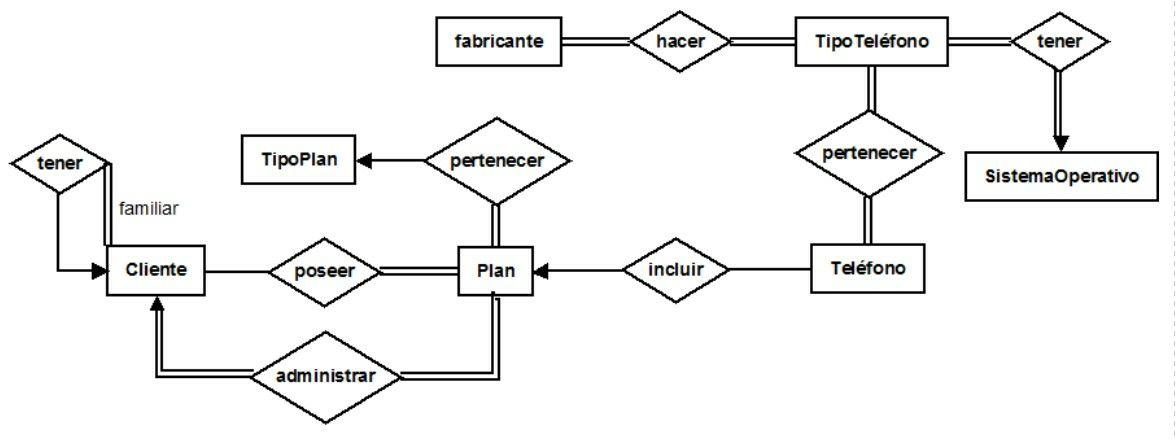
\includegraphics[scale=0.4]{./imagenes/modelo.jpg}
\end{figure}

\begin{itemize}
    % Ejercicio 1.
    \item ¿Un cliente puede tener un número ilimitado de planes?

    \textsc{Solución:} Sí. La zona rosa nos dice que hay una relación $1:m$ 
    donde \textit{un cliente tiene varios tipos de planes} ya que 
    \textit{Un plan pertence a varios tipos de plan}. Entonces, si el 
    cliente lo desea, puede llegar a tener una infinidad de planes.

    \begin{figure}[h]
        \centering
        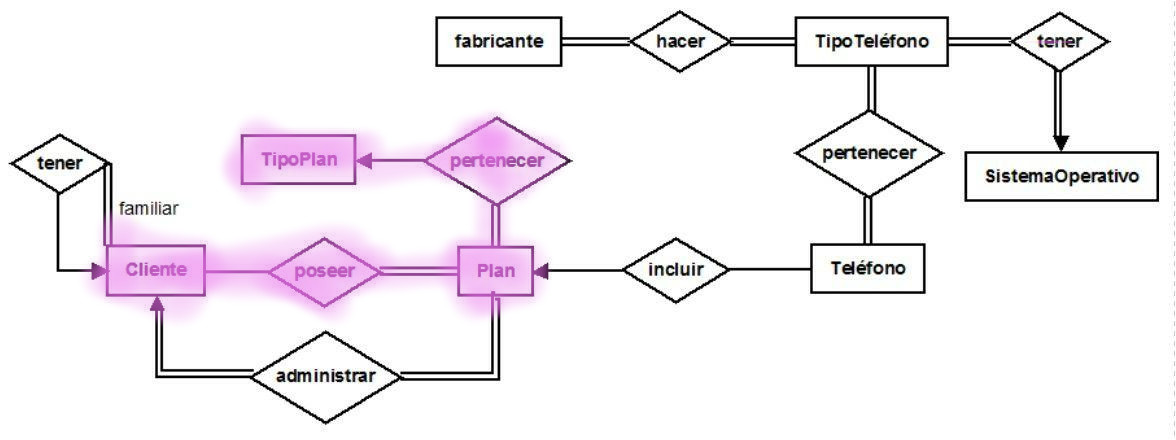
\includegraphics[scale=0.4]{./imagenes/modelo1.jpg}
    \end{figure}
    
    % Ejercicio 2.
    \item ¿Un cliente puede existir sin un plan?
    
    % Ejercicio 3.
    \item ¿Es posible crear un plan sin saber quién es el cliente?

    % Ejercicio 4.
    \item ¿El operador quiere limitar los tipos de dispositivos que se pueden 
    vincular a un tipo de plan específico?

    % Ejercicio 5.
    \item ¿Es posible mantener los datos relativos a un teléfono sin conectarlo
    a un plan?

    \textsc{Solución:}

    % Ejercicio 6.
    \item ¿Puede un teléfono puede asociar a varios planes?
    
    % Ejercicio 7.
    \item Supongamos que existe un tipo de teléfono que puede utilizar múltiples
    sistemas operativos. ¿Esta situación podría tener cabida dentro del modelo 
    incluido en la figura?

    % Ejercicio 8.
    \item ¿La empresa es capaz de realizar un seguimiento de un fabricante sin 
    mantener información sobre sus teléfonos?

    % Ejercicio 9.
    \item ¿El mismo sistema operativo se puede utilizar en mútiples tipos de  
    dispositivos? 

    \textsc{Solución:} No. La parte azul del diagrama nos muestra que la 
    relación es de uno a muchos, donde \textit{un teléfono tiene varios 
    sistemas operativos} ya que \textit{Un tipo de teléfono tiene varios 
    sistemas operativos}. 

    \begin{figure}[h]
        \centering
        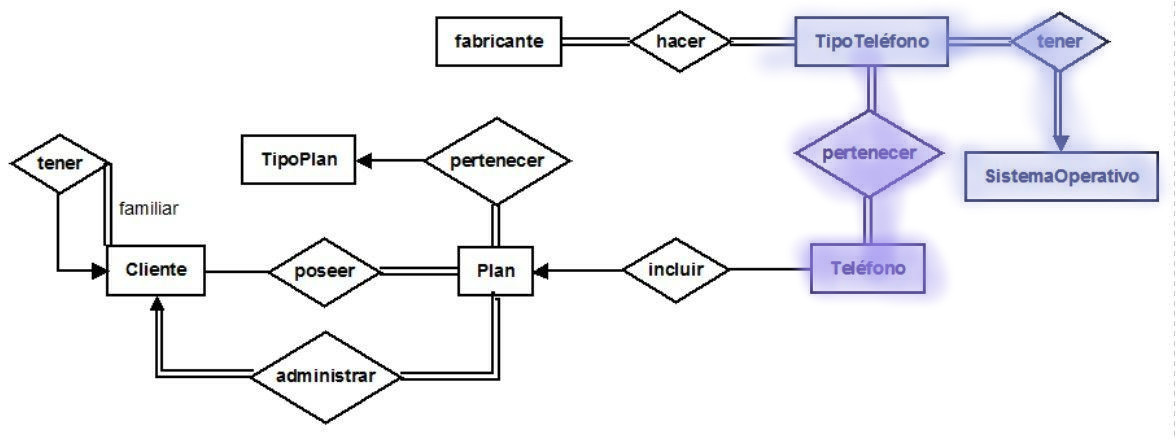
\includegraphics[scale=0.4]{./imagenes/modelo9.jpg}
    \end{figure}

    Para hacer la modificación, lo que tenemos que hacer es una relación $m:1$, 
    donde \textit{el mismo sistema operativo utiliza varios tipos de teléfono}.
    Esto se representa de la forma

    \begin{figure}[h]
        \centering
        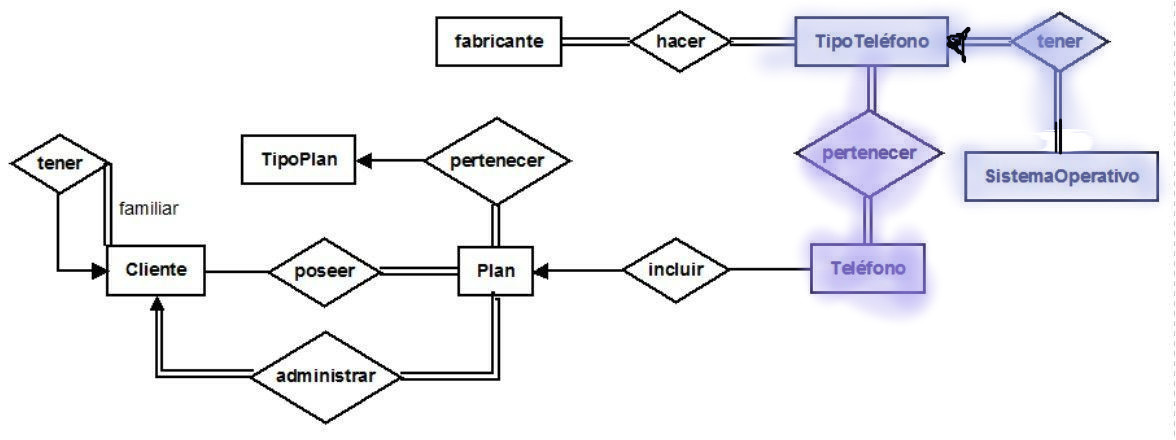
\includegraphics[scale=0.4]{./imagenes/modelo9i.jpg}
    \end{figure}

    % Ejercicio 10.
    \item Hay dos relaciones entre el Cliente y el Plan. Explicar en qué 
    difieren.

    % Ejercicio 11.
    \item Caracterizar el grado y la cardinalidad de la relación que une al 
    cliente a sí mismo. Explicar su significado.

    % Ejercicio 12.
    \item ¿Es posible vincular un teléfono a un cliente específico en un plan 
    con múltiples clientes?

    % Ejercicio 13.
    \item ¿Puede la compañía rastrear un teléfono sin identificar sus sistema 
    operativo?

\end{itemize}

\end{document}
